%%%%%%%%%%%%%%%%%%%%%%%%%%%%%%%%%%%%%%%%%%%%%%%%%%%%%%%%%%%%%%%%%%%%%%%%%%%%%%%%%%%%%%%%%%%%%%%%
%
% CS484 Written Question Template
%
% Acknowledgements:
% The original code is written by Prof. James Tompkin (james_tompkin@brown.edu).
% The second version is revised by Prof. Min H. Kim (minhkim@kaist.ac.kr).
%
% This is a LaTeX document. LaTeX is a markup language for producing 
% documents. Your task is to fill out this document, then to compile 
% it into a PDF document. 
%
% 
% TO COMPILE:
% > pdflatex thisfile.tex
%
% If you do not have LaTeX and need a LaTeX distribution:
% - Personal laptops (all common OS): www.latex-project.org/get/
% - We recommend latex compiler miktex (https://miktex.org/) for windows,
%   macTex (http://www.tug.org/mactex/) for macOS users.
%   And TeXstudio(http://www.texstudio.org/) for latex editor.
%   You should install both compiler and editor for editing latex.
%   The another option is Overleaf (https://www.overleaf.com/) which is 
%   an online latex editor.
%
% If you need help with LaTeX, please come to office hours. 
% Or, there is plenty of help online:
% https://en.wikibooks.org/wiki/LaTeX
%
% Good luck!
% Min and the CS484 staff
%
%%%%%%%%%%%%%%%%%%%%%%%%%%%%%%%%%%%%%%%%%%%%%%%%%%%%%%%%%%%%%%%%%%%%%%%%%%%%%%%%%%%%%%%%%%%%%%%%
%
% How to include two graphics on the same line:
% 
% \includegraphics[width=0.49\linewidth]{yourgraphic1.png}
% \includegraphics[width=0.49\linewidth]{yourgraphic2.png}
%
% How to include equations:
%
% \begin{equation}
% y = mx+c
% \end{equation}
% 
%%%%%%%%%%%%%%%%%%%%%%%%%%%%%%%%%%%%%%%%%%%%%%%%%%%%%%%%%%%%%%%%%%%%%%%%%%%%%%%%%%%%%%%%%%%%%%%%

\documentclass[11pt]{article}

\usepackage[english]{babel}
\usepackage[utf8]{inputenc}
\usepackage[colorlinks = true,
            linkcolor = blue,
            urlcolor  = blue]{hyperref}
\usepackage[a4paper,margin=1.5in]{geometry}
\usepackage{stackengine,graphicx}
\usepackage{fancyhdr}
\setlength{\headheight}{15pt}
\usepackage{microtype}
\usepackage{times}
\usepackage{booktabs}
\usepackage{amsmath}

% From https://ctan.org/pkg/matlab-prettifier
\usepackage[numbered,framed]{matlab-prettifier}

\frenchspacing
\setlength{\parindent}{0cm} % Default is 15pt.
\setlength{\parskip}{0.3cm plus1mm minus1mm}

\pagestyle{fancy}
\fancyhf{}
\lhead{Project Writeup}
\rhead{CS 484}
\rfoot{\thepage}

\date{}

\title{\vspace{-1cm}Homework 4 Writeup}


\begin{document}
\maketitle
\vspace{-3cm}
\thispagestyle{fancy}

\section*{Instructions}
\begin{itemize}
  \item Describe any interesting decisions you made to write your algorithm.
  \item Show and discuss the results of your algorithm.
  \item Feel free to include code snippets, images, and equations.
  \item Use as many pages as you need, but err on the short side If you feel you only need to write a short amount to meet the brief, th
  
  \item \textbf{Please make this document anonymous.}
\end{itemize}

\section*{In the beginning...}

Implementing this assignment is divided into three parts. First of all, getting interest points by calculating Harris value, secondly getting descriptors by using SIFT-like methods, and lastly matching features by calculating Euclidean distance and confidence. 
First of all, calculating the Harris value is useful to find out the interest points. As written below in equation \ref{eq:one}, Harris matrix is given using the partial determinants. Harris value could be calculated as given under from equation \ref{eq:two}. 

\begin{equation}
A = \sum_{u} \sum_{v} w(u,v) 
    \begin{bmatrix}     I_x^2 & I_xI_y \\         I_xI_y & I_y^2     \end{bmatrix} 
\label{eq:one}
\end{equation}
\begin{equation}
h = det(A) - \alpha * tr^2(A)
\label{eq:two}
\end{equation}

As suggested from the textbook by Szleski, alpha is recommended as 0.06


To discuss about SIFT-like progress, dividing into 16 cells and calculate each of the gradient values for 8 directions, adding up from all values inside the cell is needed. 

For understanding the implementation detail written below, we should have a look on Sobel filter. Sobel filter is used to approximately calculate the derivatives for both x and y axis, easily can both calculate magnitude and angle.

To add on, we should use NNDR (Nearest Neighbor Distance Ratio) to calculate as confidences. The equation \label{eq:three} is written as below, d1 is the nearest neighbor distance, d2 is the second nearest neighbor distance. 

\begin{equation}
NNDR = d_1 / d_2
\label{eq:three}
\end{equation}

\section*{Interesting Implementation Detail}

- get interest points


I made up with two different Gaussian filters, large one with width of 9 and sigma of 2, small one with width of 3 and sigma of 1. Two Gaussian filters would improve blurring. To calculate both gradients of x and y axis, I used sobel filters and made convolution. It is implemented as below

\begin{lstlisting}[style=Matlab-editor]
% small, large gaussian filter -> sigma 2, 1 for each large, small filter
large_gaussian = fspecial('gaussian',9,2);
small_gaussian = fspecial('gaussian',3,1);

% gradient values of small-gaussian-filtered image
new_image = imfilter(image,small_gaussian);
image_db=im2double(new_image);
sobely= [1 ,0 ,-1; 2,0,-2; 1, 0 ,-1];
sobelx= [1,2,1; 0,0, 0; -1, -2 ,-1];
x_grad = conv2(image_db,sobelx,'same');
y_grad = conv2(image_db,sobely,'same');

% calculate grads : filter with large gaussian filter 
xy_grad = y_grad .* x_grad;
xy_grad = imfilter(xy_grad, large_gaussian); 
xx_grad = x_grad .* x_grad; 
xx_grad = imfilter(xx_grad, large_gaussian); 
yy_grad = y_grad .* y_grad;
yy_grad = imfilter(yy_grad, large_gaussian); 

\end{lstlisting}

- get descriptors


To calculate gradient values for all 8 directions, I made 8 different sobel filters. After it, filtering with Gaussian filter blurred the picture and made it better to calculate.

\begin{lstlisting}[style=Matlab-editor]
% Use sobel filter to rotate image in certain direction and calculate gradient  
filter = [];
m = fspecial('sobel'); 
filter(:,:,1) = m;
for i=2:8 
    % rotating sobel filter 45 degrees from former one
    m = [m(4) m(7) m(8); m(1) m(5) m(9); m(2) m(3) m(6)];
    filter(:,:,i) = m;
end

% new_image is an image containing 8 copies of images filtered by 8 sober
% filters
new_image = zeros(image_size(1),image_size(2),8); 
for i=1:8 
    new_image(:,:,i) = imfilter(image,filter(:,:,i)); 
end

% filter with gaussian, sigma = half_width
gauss_filter = fspecial('gaussian', [half_width, half_width], half_width);
new_image = imfilter(new_image, gauss_filter);


\end{lstlisting}

- match features

As mentioned before, matching features will calculate confidences using NNDR, used find function and flipped it after finding. 

\begin{lstlisting}[style=Matlab-editor]
% confidences > 1
[B,I] = sort(K,2);
neighbor1 = B(:,1);
neighbor2 = B(:,2);
confidences = neighbor1 ./ neighbor2;

% use find
i = find(confidences)
s = size(i);
matches = zeros(s(1),2);
matches(:,1) = i; 
matches(:,2) = I(i);

% confidences in correct value
confidences = 1./confidences(i)

\end{lstlisting}


\section*{A Result}

Three pictures after three functions are described under as figure \label{fig:result1} and the accuracy was 86\%, 96\%, 3\% for the best 100 points.

\begin{figure}[h]
    \centering
    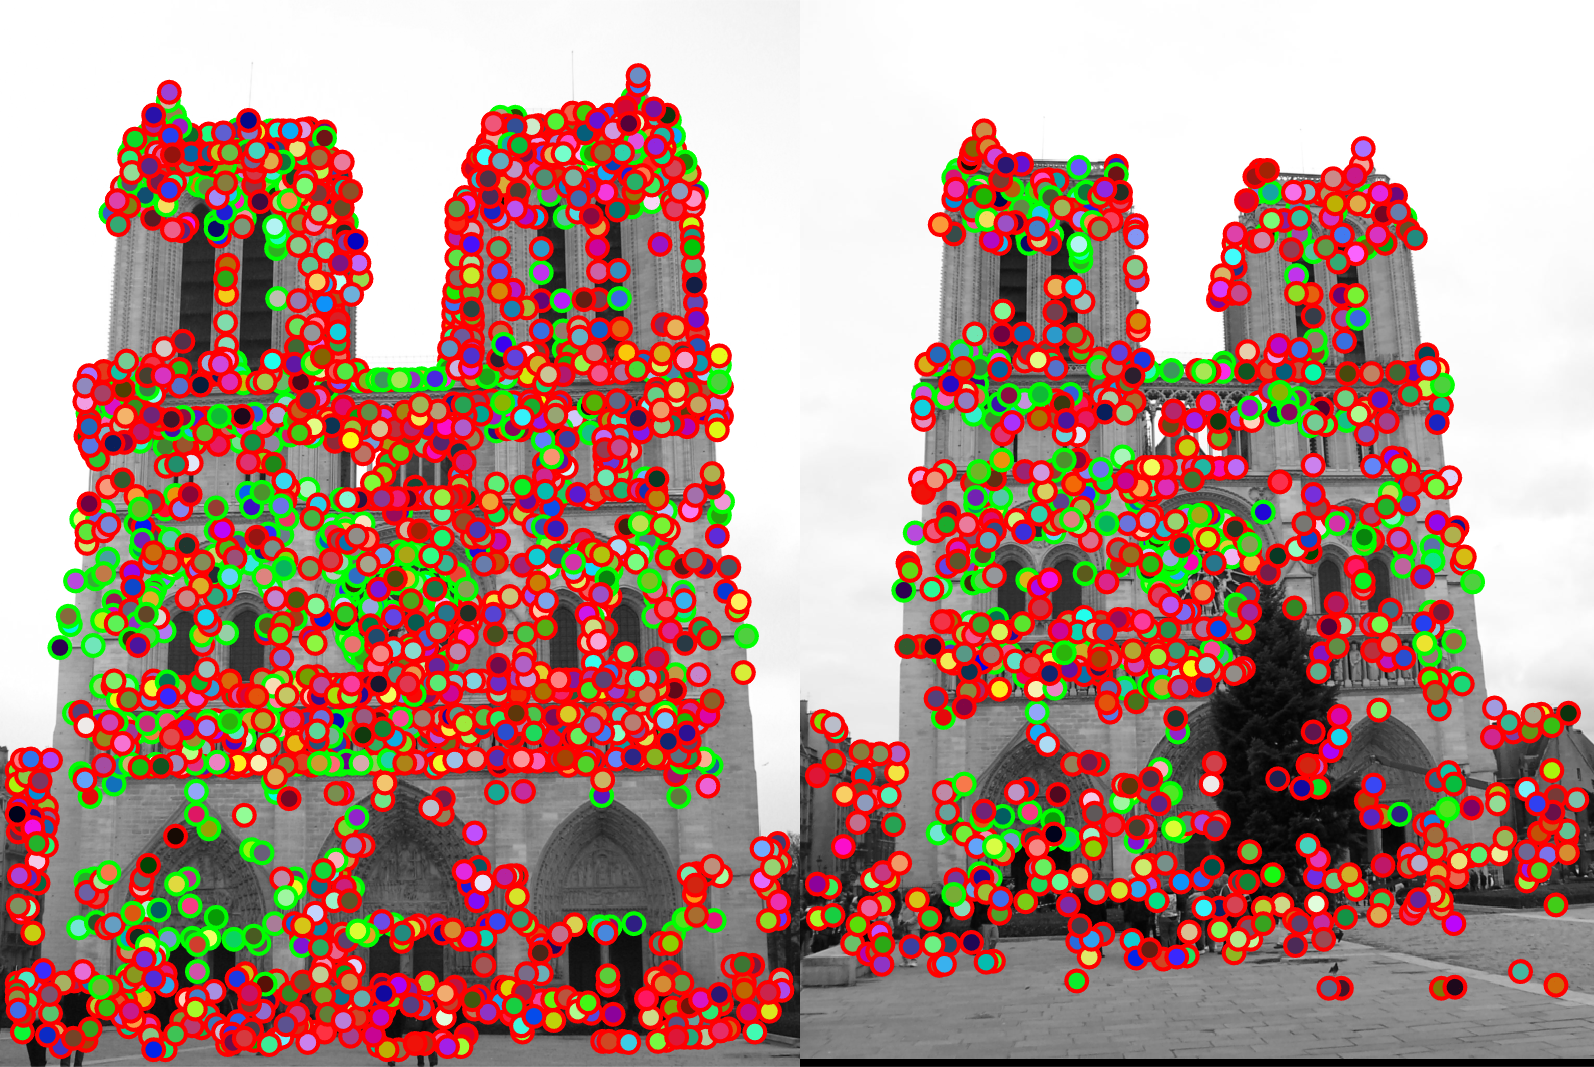
\includegraphics[width=3cm]{../code/eval_ND.png}
    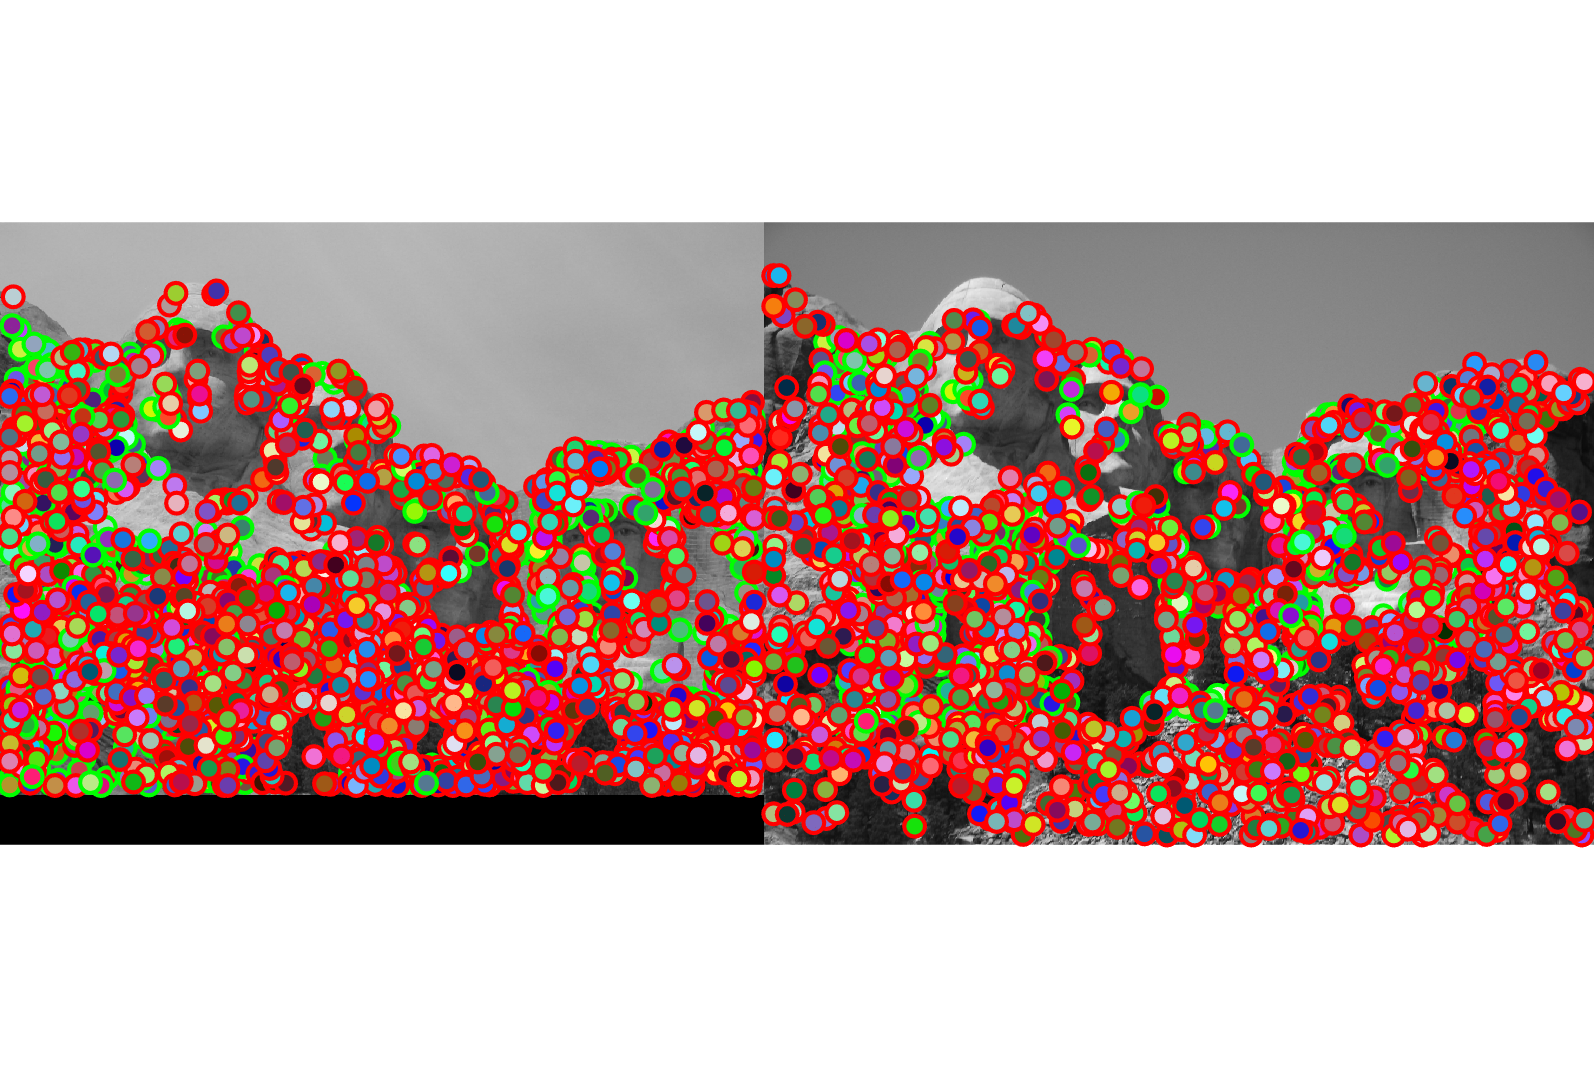
\includegraphics[width=3cm]{../code/eval_MR.png}
    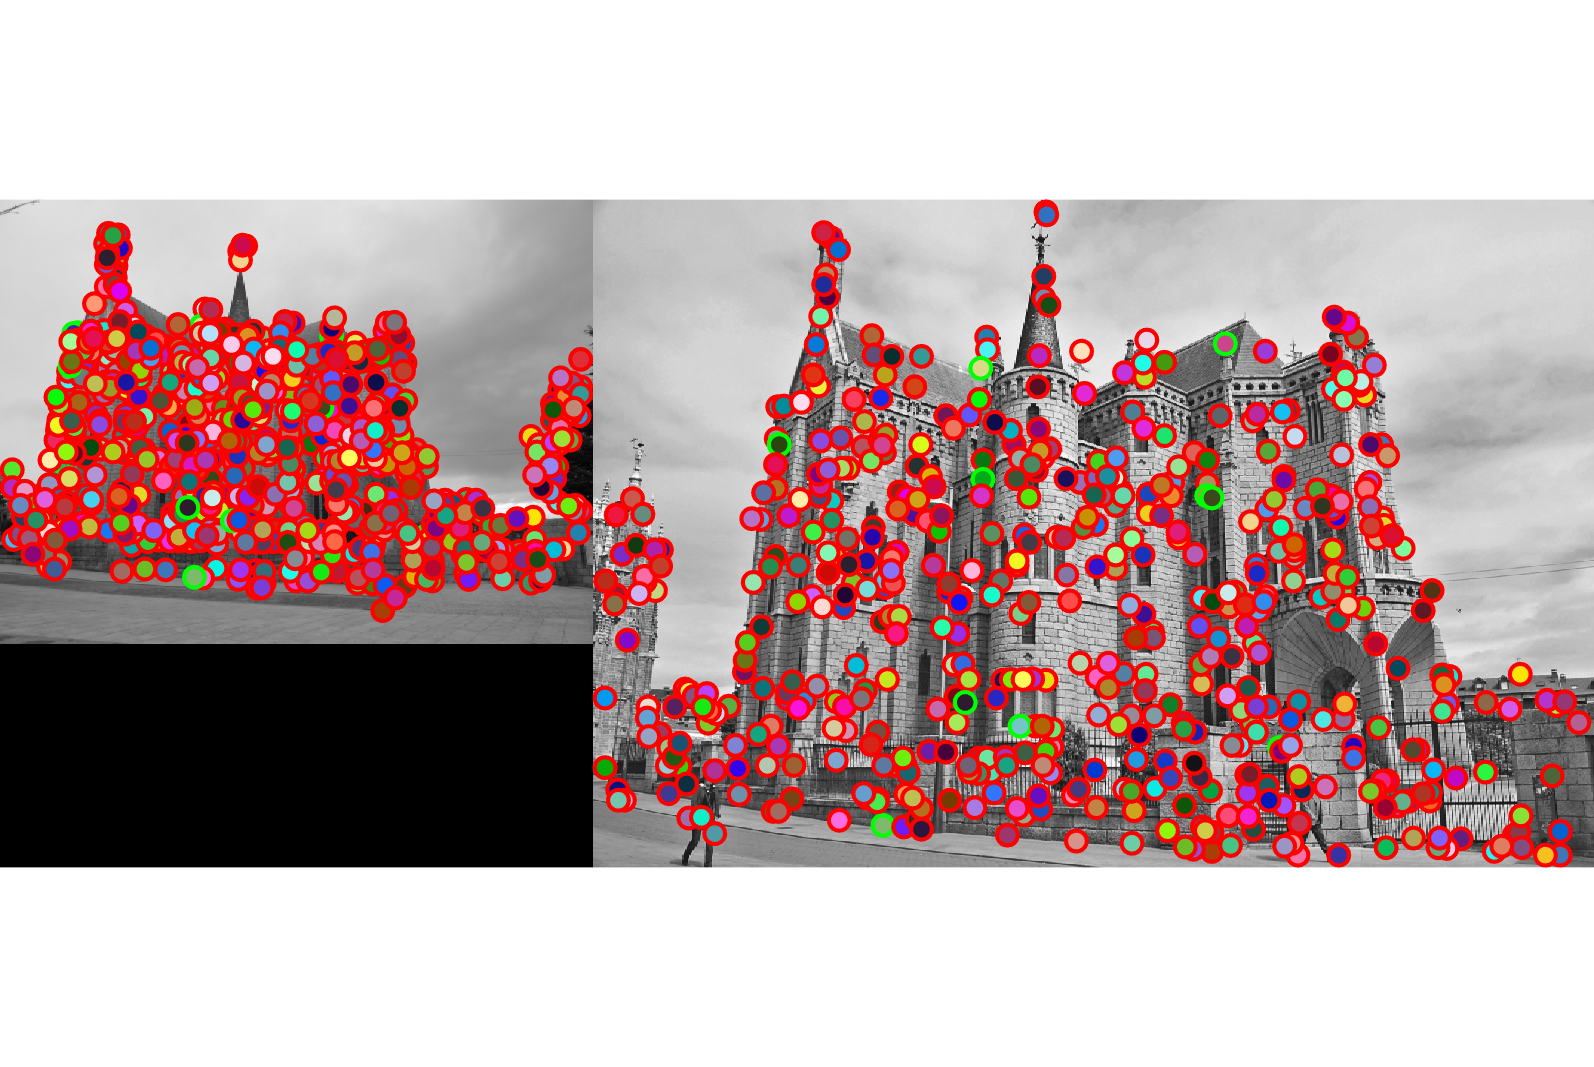
\includegraphics[width=3cm]{../code/eval_EG.png}
    \caption{\emph{Left:} Notre Dame de Paris \emph{Center:} Mount Rushmore \emph{Right:} Gaudi's Episcopal Palace}
    \label{fig:result1}
\end{figure}


\end{document}
